\documentclass[UTF8,fontset=fandol,a4paper,11pt]{ctexart}

\usepackage{geometry}
\usepackage{booktabs}
\usepackage{array}
\usepackage{tabularx}
\usepackage{graphicx}
\usepackage{amsmath}
\usepackage{amssymb}
\usepackage{newtxtext}
\usepackage{newtxmath}
\usepackage{xcolor}
\usepackage{caption}
\usepackage{enumitem}
\usepackage{hyperref}
\usepackage{placeins}
\usepackage{float}

\geometry{left=2.4cm,right=2.4cm,top=2.5cm,bottom=2.5cm}
\setlength{\emergencystretch}{2em}
\clubpenalty=10000
\widowpenalty=10000
\displaywidowpenalty=10000
\ctexset{
  section = {
    format = \centering\Large\bfseries\heiti
  },
  subsection = {
    format = \large\bfseries\heiti
  },
  subsubsection = {
    format = \normalsize\bfseries\heiti
  }
}
\hypersetup{hidelinks}
\captionsetup{font=small,labelfont=bf}
\setlength{\tabcolsep}{5pt}
\renewcommand{\arraystretch}{1.12}
\newcolumntype{Y}{>{\raggedright\arraybackslash}X}

\newcommand{\method}{HMSA}

\title{\heiti\bfseries 共识预测与多评分者分布辅助学习：\\教育回答自动评审中的受控实证研究}
\author{匿名投稿\\作者信息将在录用后补充}
\date{}

\begin{document}
\pagestyle{plain}
\maketitle

\begin{abstract}
教育回答通常由多名评分者共同标注，但自动评审模型往往只学习聚合后的单一等级，未利用评分分布中保留的人类判断差异。直接以该分布训练部署输出头，又可能改变整数评分所对应的决策目标。本文将软标签辅助多任务学习范式应用于教育五级评分，构建 Hard-Main/Soft-Auxiliary（HMSA）配置：硬标签主头与评分分布辅助头共享主干；模型选择、最终整数评分和正文评价指标均由硬标签主头给出，辅助头不参与评分决策。与数据、主干、优化设置及评分路径均匹配的 Hard-only 基线相比，HMSA 在三个随机种子上将测试 MAE 从 $0.433\pm0.009$ 降至 $0.388\pm0.003$，将精确匹配率从 $0.731\pm0.001$ 提升至 $0.749\pm0.002$，并将 Kendall $\tau_b$ 从 $0.561\pm0.018$ 提升至 $0.611\pm0.004$。分等级分析显示，1--4 分召回率均有提高，5 分召回率仅轻微下降；低分回答被严重高估的错误数在三个种子的平均结果中也下降。为缩小机制解释，本文补充两项仅使用训练集和开发集的事后对照：标签内置换破坏样本--评分分布对应关系，MeanAux 则在相同双头结构下用连续人类均分与 Smooth L1 替代分布交叉熵。HMSA 相比 MeanAux 的开发集 MAE、精确匹配率和 Kendall $\tau_b$ 分别改善 0.016、0.021 和 0.028，且三个种子均同向。由于经验分布与连续均分在当前数据中一一对应，该结果支持目标表示与损失几何影响训练效果，但不能解释为分布包含了均分之外的额外标签信息；两项机制对照均属事后开发集证据，仍需独立数据确认。
\end{abstract}

\noindent\textbf{关键词：} 教育大语言模型；自动评审；多评分者监督；软标签；多任务学习

\section{引言}

大语言模型日益用于教育内容生成、智能辅导和自动质量控制，由此产生了对大规模、稳定且与人类判断一致的自动评审器的需求。EduBench 等教育评价数据集通常为每个“问题--回答--评价维度”条目收集多位评分者的判断，并将其聚合为一个 1--5 分标签，供模型训练和比较\cite{edubench}。聚合标签提供了明确的分类目标，却压缩了人类标签变异\cite{plank2022,davani2022}：评分模式 $[4,4,4]$ 与 $[3,4,4]$ 的硬标签均为 4，但前者表示完全一致，后者仍在 3 分上保留三分之一的经验概率质量。

一种自然做法是令分类头直接拟合经验评分分布。然而，部署时仍须输出一个整数分数；当同一输出头兼顾分布拟合与硬决策时，其优化目标与部署目标不再完全一致。已有研究提出将聚合标签预测作为主任务、将标注分布预测作为辅助任务的软标签多任务范式\cite{fornaciari2021}。本文关注该范式在教育五级评分中的适配问题：多评分者分布应替代硬标签目标、与硬标签在同一输出头中混合，还是作为独立辅助任务约束共享表示？

为此，本文首先以单个随机种子诊断直接软目标（Direct-soft）和单头硬软混合目标（Single-head mix）；两种配置均未通过预先设定的开发集推进门槛。随后构建 Hard-Main/Soft-Auxiliary（HMSA）配置：共享主干连接两个参数独立的线性头，硬标签主头负责模型选择与最终预测，评分分布辅助头为训练提供附加约束但不参与评分决策。两项损失共同更新共享主干，部署时可只保留硬标签主头。除匹配基线比较外，本文还以标签内置换和连续均分辅助目标两项开发集对照，分别考察样本级对应、一般双头正则化与目标表示方式。核心问题是：\emph{在保持硬标签评分路径不变的条件下，多评分者分布辅助任务能否改善匹配基线，其收益与代价分布在哪里，以及哪些开发集证据能够缩小其机制解释？}

\paragraph{与既有教育评审研究的联系。}
相关审计研究《Auditing Large Language Models as Educational Assistants and Judges》从生成模型排名、学科与评价维度差异以及自动评审器--人类评分一致性等角度分析教育大模型，并将 0.6B EduBenchEvaluator 作为任务专用评审器\cite{prioraudit}。其中观察到的低分识别不足与系统性高估构成本文的任务动机。本文沿用该教育评分任务与基座评审器，将研究问题收敛为监督设计：在保留整数评分接口的前提下，三位评分者的分布信息应如何进入训练。既有结果用于说明任务背景；本文的方法增益均依据当前固定划分上重新训练且配置匹配的 Hard-only 基线计算。

本文的主要贡献如下：

\begin{itemize}[leftmargin=2em]
  \item 在教育回答五级评分任务中，受控比较聚合硬标签、直接评分分布监督、单头硬软混合和硬主头--软辅助头配置；HMSA 在不改变最终评分路径的情况下，使三个随机种子的 MAE、精确匹配率与 Kendall $\tau_b$ 均同向改善。
  \item 增加两项三种子开发集机制对照：标签内置换仅破坏训练样本与评分分布的对应关系，MeanAux 则在保持双头结构、参数量和硬头评分路径不变时，以连续人类均分替代分布辅助目标。HMSA 对两项对照均取得一致主指标优势，分别支持样本级对应和目标表示--损失设计提供增量；由于均分与分布一一对应，本文不作额外标签信息主张。
  \item 从总体指标、低分到高分严重误判（L2H）、分等级召回率以及评分一致性分层刻画收益与代价，并采用单种子诊断、三种子评估、检查点重载复算和测试前配置锁定区分不同证据层级。
\end{itemize}

\section{相关工作}

\subsection{教育场景中的自动评审}

LLM-as-a-judge 已成为开放式生成评价的重要工具\cite{zheng2023mtbench}。教育评价还需要同时考虑学习科学维度、学生错误和任务特定评分标准；MRBench 与 MathTutorBench 因而引入多维教学评价、人工标注及任务专用评审模型\cite{maurya2025mrbench,macina2025mathtutorbench}。已有研究同时表明，通用 LLM 评审器可能具有位置偏差、自偏好和过度自信等问题\cite{gu2024survey,li2024llmjudge,wang2025overconfidence}。因此，本研究不重新比较不同规模的提示式评审器，而是在固定的 0.6B 任务专用评审器中检验多评分者监督的放置方式及其误差特征。

\subsection{人类标签变异与多评分者监督}

聚合标签可能掩盖主观判断、多个合理解释或系统性评分差异\cite{plank2022,davani2022}。学习评分分布可保留少数意见，并避免把所有样本表示为完全确定的独热目标\cite{peterson2019human,uma2021learning}。LeWiDi 系列共享任务进一步推动了保留多重标注及使用软标签指标的统一评测\cite{lewidi2021,lewidi2023}。不过，多评分者变化并不都等价于有效分歧，也可能包含标注误差。下文统一使用“多评分者分布”描述训练目标，而不预设其全部概率质量均对应可解释的认知分歧。

\subsection{软标签辅助多任务学习}

多任务学习允许主任务保持部署目标，同时由相关辅助任务对共享参数提供附加训练约束\cite{caruana1997multitask}。Fornaciari 等提出软标签多任务学习：以聚合标签预测为主任务，以标注分布预测为辅助任务，并共享神经表示\cite{fornaciari2021}。其总体范式与 HMSA 高度相关。后续大规模人类标签变异研究将软标签和多数投票标签的共享编码器多任务配置纳入标准比较，并在六个数据集、十四种训练方法上进行系统评估\cite{kurniawan2026}。本文的增量不在于提出通用双头结构，而在于研究五级教育序数评分中的部署约束，比较软监督的三种放置方式，并联合评估连续人类均分误差、低分高估、分等级召回和硬头独立部署。进一步地，标签内置换对照固定类别条件软目标组成，只改变样本级对应关系；MeanAux 则在匹配双头容量下替换辅助目标与损失，分别用于缩小“样本对应”“目标表示--损失设计”与“一般辅助正则化”之间的解释空间。

表\ref{tab:positioning} 进一步概括本文与最相关范式的关系：结构思想是继承的，新增证据集中于教育序数评分、监督放置对照、部署接口与风险分层。

\begin{table}[H]
\centering
\caption{本文与 Fornaciari 等（2021）soft-label multi-task 范式的定位比较。}
\label{tab:positioning}
\small
\begin{tabularx}{\linewidth}{@{}>{\raggedright\arraybackslash}p{0.16\linewidth}YY@{}}
\toprule
维度 & Fornaciari 等（2021） & 本文 \\
\midrule
共同结构 & 硬标签主任务与分布辅助任务共享编码器 & 沿用硬主头--软辅助头共享主干 \\
任务设置 & 词性标注、词干分类 & 教育回答 1--5 级序数评分 \\
核心问题 & 利用标签分歧改进预测 & 比较三种软监督放置方式 \\
损失设计 & 主任务与辅助分布损失等权联合 & 硬标签 CE 与分布 CE 等权联合 \\
评分接口 & 主任务头输出标签 & 仅由硬头输出整数分数 \\
证据重点 & 2 项 NLP 任务、3 个数据集、3 种辅助损失 & 序数指标、风险分层、置换与均分对照 \\
\bottomrule
\end{tabularx}
\end{table}


\section{任务定义与研究问题}

每个样本 $i$ 的输入 $x_i$ 由问题、生成回答和评价维度拼接而成。三位人类评分者给出 $r_{ij}\in\{1,2,3,4,5\}$，其中 $j\in\{1,2,3\}$。连续人类均分与聚合硬标签分别定义为
\begin{equation}
\bar r_i=\frac{1}{3}\sum_{j=1}^{3}r_{ij},\qquad
y_i=\operatorname{round}(\bar r_i)\in\{1,\ldots,5\}.
\end{equation}
在所用划分中，三人评分模式只有完全一致或相邻等级 2:1 两类，因此 $y_i$ 也与经验分布的众数一致。进一步审计显示，训练集与开发集均出现 13 个连续均分取值和 13 种经验分布，测试集出现 11 个均分取值和 11 种经验分布；在三个划分内，$\bar r_i$ 与评分多重集均一一对应。因此，当前数据不能用于证明完整分布比连续均分包含更多标签信息，二者的差异只能体现目标表示和训练损失的差异。软目标为
\begin{equation}
d_{ik}=\frac{1}{3}\sum_{j=1}^{3}\mathbb{I}(r_{ij}=k),\qquad k\in\{1,\ldots,5\}.
\end{equation}
例如，$[4,4,4]$ 对应 $d=(0,0,0,1,0)$，而 $[3,4,4]$ 对应 $d=(0,0,\frac{1}{3},\frac{2}{3},0)$；二者聚合标签均为 4，但后者保留了边界分歧。

本文回答三个研究问题：

\begin{itemize}[leftmargin=2em]
  \item \textbf{RQ1：} 在匹配的训练与评测条件下，将经验评分分布放入独立辅助任务，能否改善硬标签基线？
  \item \textbf{RQ2：} 收益和代价分布在哪些总体指标、分数等级及严重错误类型中？
  \item \textbf{RQ3：} 在保持硬头部署路径和双头容量不变时，HMSA 的开发集增量能否由一般辅助正则化、打乱后的类别条件软目标或连续均分辅助目标复现？
\end{itemize}

\section{方法}

\subsection{匹配硬标签基线}

硬标签基线 Hard-only 使用 Qwen3-Reranker-0.6B 的序列分类路径\cite{qwen3embedding}。主干输出的最后一个非填充词元表征经无偏置线性层映射为五类逻辑值（logits）$z_i^{(h)}$，训练损失为
\begin{equation}
\mathcal{L}_{\mathrm{hard}}=-\log \operatorname{softmax}(z_i^{(h)})_{y_i}.
\end{equation}
预测结果始终为
\begin{equation}
\hat y_i=\operatorname*{argmax}_{k\in\{1,\ldots,5\}}z_{ik}^{(h)}.
\end{equation}
Hard-only 不使用三位评分者的个体分数。

\subsection{诊断性单头软监督}

为区分“使用软标签”与“软标签放在哪里”，实验先固定两个单头诊断配置。令
$p_{ik}=\operatorname{softmax}(z_i)_k$。Direct-soft 直接用经验分布训练部署输出头：
\begin{equation}
\mathcal{L}_{\mathrm{direct}}=-\sum_{k=1}^{5}d_{ik}\log p_{ik}.
\end{equation}
Single-head mix 在同一组部署 logits 上使用混合目标
\begin{equation}
t_i=0.5\,\operatorname{onehot}(y_i)+0.5\,d_i,
\qquad
\mathcal{L}_{\mathrm{mix}}=-\sum_{k=1}^{5}t_{ik}\log p_{ik}.
\end{equation}
两者推理时均对该单头取最大概率类别，因此软目标直接约束部署逻辑值。两种配置仅以随机种子 42 进行推进诊断，具体开发集结果见附录表\ref{tab:diagnostic_seed42}，不构成多种子消融。

\subsection{HMSA：硬主头与软辅助头}

如图\ref{fig:architecture} 所示，HMSA 将软标签辅助多任务思想\cite{fornaciari2021}应用于教育五级评分，并规定最终评分只读取硬标签主头。该配置在同一主干上增加一个参数独立的线性辅助头。为避免额外随机初始化成为混杂因素，软头由初始硬头深拷贝得到，两者初始权重完全相同。软头逻辑值记为 $z_i^{(s)}$，其交叉熵为
\begin{equation}
\mathcal{L}_{\mathrm{soft}}=-\sum_{k=1}^{5}d_{ik}\log \operatorname{softmax}(z_i^{(s)})_k.
\end{equation}
总损失固定为
\begin{equation}
\mathcal{L}_{\mathrm{HMSA}}=\mathcal{L}_{\mathrm{hard}}+\lambda\mathcal{L}_{\mathrm{soft}},\qquad \lambda=1.0.
\end{equation}
辅助损失权重固定为 $\lambda=1.0$，不进行搜索。两项损失均反向传播到共享主干，因此辅助任务仍会影响硬任务表征；两个输出目标仅在参数独立的头中分离。冻结评测程序同时记录软头诊断量，但模型检查点选择、最终预测和正文报告的评分指标只读取硬头；两个头不进行平均，辅助头不参与测试评分决策。

\begin{figure}[htbp]
\centering
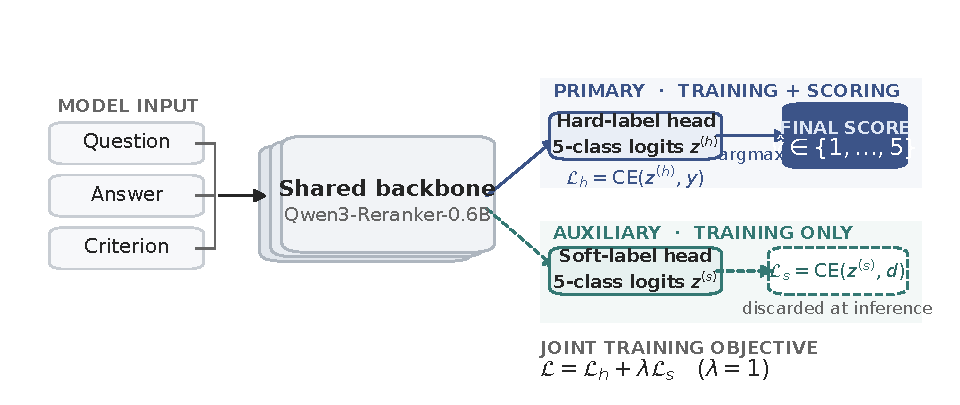
\includegraphics[width=0.98\linewidth]{figures/fig1_hmsa_architecture.pdf}
\caption{HMSA 的训练与评分路径。深蓝色实线表示训练和最终评分均使用的硬标签主路径，青绿色虚线表示仅在训练时提供约束的评分分布辅助路径；两项损失共同更新共享主干，推理时丢弃辅助分支并只保留硬标签主头。}
\label{fig:architecture}
\end{figure}

\subsection{标签内打乱软目标机制对照}

本文构造标签内置换对照（Shuffled-soft），用于检验 HMSA 的收益是否仅来自增加辅助头或提供类别层面的软目标先验。令训练集中硬标签为 $k$ 的索引集合为 $\mathcal{I}_k$，并在每个集合内固定一个双射 $\pi_k:\mathcal{I}_k\rightarrow\mathcal{I}_k$。对样本 $i\in\mathcal{I}_k$，辅助头的训练目标替换为
\begin{equation}
\tilde d_i=d_{\pi_k(i)}.
\end{equation}
该置换保持每个硬标签内软目标的完整多重集及其熵分布，因而也保持软目标众数与硬标签的一致性；改变的只有哪一个训练样本接收哪一个细粒度评分分布。输入、硬标签、双头结构、头部初始化、损失权重、优化器、检查点规则与硬头推理路径均与 HMSA 相同。开发集仍使用原始未打乱的人类评分，三个模型种子共享同一份固定映射。

映射由固定种子 20260730 确定。在 2,654 个训练条目中，1,490 个条目的五维软目标实际改变，占 56.14\%；其余条目在置换后获得相同离散分布。该对照在主实验完成后补充，仅使用训练集和开发集，因此用于比较原始对应关系与类别条件软监督，证据属性为事后探索性分析。

\subsection{连续均分辅助目标对照}

为检验 HMSA 的收益是否可由任意细粒度人类目标复现，本文进一步构造 MeanAux。该配置保留 HMSA 的共享主干、硬标签主头和一个由初始硬头深拷贝得到的五分类逻辑值辅助头，因此辅助参数量与初始化方式均匹配。令
\begin{equation}
q_{ik}^{(m)}=\operatorname{softmax}(z_i^{(m)})_k,
\qquad
\mu_i=\sum_{k=1}^{5}kq_{ik}^{(m)},
\end{equation}
其中 $\mu_i$ 是辅助头的期望分数。MeanAux 以连续人类均分 $\bar r_i$ 为目标，使用 $\beta=1$ 的 Smooth L1 损失：
\begin{equation}
\mathcal{L}_{\mathrm{mean}}=
\operatorname{SmoothL1}_{\beta=1}(\mu_i,\bar r_i),
\qquad
\mathcal{L}_{\mathrm{MeanAux}}=
\mathcal{L}_{\mathrm{hard}}+\mathcal{L}_{\mathrm{mean}}.
\end{equation}
辅助权重固定为 1.0，不搜索损失权重、$\beta$ 或训练轮数。模型选择和全部评分指标仍只读取硬头。由于当前三个划分内经验分布与连续均分一一对应，MeanAux 与 HMSA 的比较控制了标签信息的可恢复性，但同时改变目标参数化与损失函数；因此它检验哪种训练目标在当前设定中更有效，不能单独区分分类概率几何与交叉熵梯度的作用。

表\ref{tab:method_matrix} 汇总了 Hard-only、两个诊断性单头配置、两项事后机制对照与 HMSA 之间的监督和推理差异。

\begin{table}[H]
\centering
\caption{六种监督配置。Direct-soft 与 Single-head mix 为随机种子 42 的诊断配置；Shuffled-soft 与 MeanAux 为事后开发集机制对照。}
\label{tab:method_matrix}
\small
\setlength{\tabcolsep}{3pt}
\begin{tabularx}{\linewidth}{@{}lYYcYcY@{}}
\toprule
配置 & 主头目标 & 辅助头目标 & 头数 & 推理 & 种子 & 证据角色 \\
\midrule
Hard-only & 聚合硬标签 & -- & 1 & 硬头 & 42/43/44 & 匹配基线 \\
Direct-soft & 三人经验分布 & -- & 1 & 同一头 & 42 & 诊断实验 \\
Single-head mix & 硬/软目标各 0.5 & -- & 1 & 同一头 & 42 & 诊断实验 \\
Shuffled-soft & 聚合硬标签 & 标签内置换 & 2 & 仅硬头 & 42/43/44 & 事后机制对照 \\
MeanAux & 聚合硬标签 & 连续人类均分 & 2 & 仅硬头 & 42/43/44 & 事后目标对照 \\
HMSA & 聚合硬标签 & 三人经验分布 & 2 & 仅硬头 & 42/43/44 & 三种子评估 \\
\bottomrule
\end{tabularx}
\end{table}


\FloatBarrier
\section{实验设计}

\subsection{数据与输入}

实验沿用固定数据划分，训练集、开发集和测试集分别包含 2,654、664 和 2,218 个条目。本文比较的所有配置使用完全相同的数据行与输入。模型输入仅包含清洗后的问题、生成回答和评价维度，不加入学科、教育层级、生成模型身份、评分细则或自动评审器分数。

所有配置使用完全相同的输入模板，其中花括号内容由相应字段替换：
\begin{quote}
\small\ttfamily
Question:\\
\{question\}\\[0.35em]
Answer:\\
\{answer\}\\[0.35em]
Evaluation Dimension:\\
\{metric\}\\[0.35em]
Predict the human-aligned educational quality score from 1 to 5.
\end{quote}

训练集中三人一致样本为 1,169 条，相邻等级 2:1 分歧样本为 1,485 条；开发集分别为 291 和 373 条。训练标签分布为 1--5 分分别 24、52、251、946、1,381 条，测试集分别为 56、47、194、720、1,201 条。鉴于低分样本明显较少，除总体指标外还单独报告 1、2 分召回率和 L2H 严重错误。为保持 Hard-only 与 HMSA 的单变量比较，实验未采用重采样或类别权重。

固定划分及各等级样本数见表\ref{tab:data_distribution}。

\begin{table}[H]
\centering
\caption{固定数据划分及硬标签分布。}
\label{tab:data_distribution}
\small
\begin{tabular}{lrrrrrr}
\toprule
划分 & $n$ & 1 分 & 2 分 & 3 分 & 4 分 & 5 分 \\
\midrule
训练集 & 2,654 & 24 & 52 & 251 & 946 & 1,381 \\
开发集 & 664 & 6 & 14 & 62 & 237 & 345 \\
测试集 & 2,218 & 56 & 47 & 194 & 720 & 1,201 \\
\bottomrule
\end{tabular}
\end{table}


\subsection{训练配置与受控变量}

Hard-only、HMSA、Shuffled-soft 与 MeanAux 均训练 10 轮，最大序列长度为 2,048。AdamW 优化器的学习率为 $2\times10^{-5}$、权重衰减为 0.01，余弦调度器的预热比例为 0.05。微批量大小为 4，梯度累积步数为 32，有效批量大小为 128，梯度范数裁剪阈值为 1.0。配对比较采用随机种子 42、43 和 44。每轮训练后在开发集上评估，选择硬标签精确匹配率最高的模型检查点；并列时保留更早轮次。除独立软头及其损失外，HMSA 与 Hard-only 的数据、输入、主干、硬头路径、优化设置、训练轮数、模型选择和推理规则完全一致；Shuffled-soft 相比 HMSA 只改变训练样本与软目标的对应关系，MeanAux 则只替换辅助目标及相应损失。

基座模型与分词器从同一本地 Qwen3-Reranker-0.6B 快照加载，使用 Hugging Face 序列分类路径、动态批量填充和长度 2,048 截断。输入审计显示，训练集和开发集的最长序列分别为 1,265 和 1,269 个词元，实际未发生截断。训练脚本采用自动混合精度配置，并启用梯度检查点，对主干与输出头进行完整参数微调。分类表示取最后一个非填充词元；两个五分类头均为无偏置线性层。HMSA 和 MeanAux 相比 Hard-only 均仅新增一个含 5,120 个参数的辅助头，约占 0.6B 名义规模的 0.0009\%。三个随机种子的训练日志显示，Hard-only、HMSA 与 MeanAux 的平均单次训练耗时分别为 43.26、43.23 和 47.13 分钟，峰值已分配显存均约为 6.06 GB。部署时可裁剪辅助头；裁剪后的评分路径和参数量与 Hard-only 相同。

实验产物记录了训练源码提交 \texttt{193d64e5}、运行提交 \texttt{4e95b0a4} 与本地模型路径，但未单独保存自动混合精度的最终解析值、上游模型和分词器版本、精确的 PyTorch/Transformers 版本以及 GPU 型号。本文不补写无法验证的信息，并将该缺口列为复现限制。

\subsection{分阶段证据协议}

正式实验依次执行单种子诊断、三种子开发集评估、六个模型检查点重载复算和测试集评测。Direct-soft 与 Single-head mix 仅使用随机种子 42，并在未通过预先设定的开发集门槛后停止，因而不提供多种子统计证据。HMSA 通过该门槛后，才使用随机种子 42、43 和 44 进行开发集评估。推进条件包括：MAE 至少在两个种子上改善、精确匹配率非劣、平均 MAE 至少降低 0.005，且排序指标和高分等级召回率不得明显退化。全部 11 项检查通过后，重新加载 Hard-only 与 HMSA 的六个模型检查点，复算开发集预测，并核对文件哈希、所选轮次和指标。全部检查点选择与实验配置均基于开发集确定；规则锁定后，在同一正式评测流程中计算 Hard-only 与 HMSA 三个种子的测试结果。测试结果不用于选择轮次、修改结构或搜索当前实验的超参数。

Shuffled-soft 与 MeanAux 均在上述正式流程完成后新增，且只在训练集上训练、在开发集上完成模型选择与评测，未生成测试预测。MeanAux 最初设置了随机种子 42 的计算节约门槛；因三个种子采用并行执行，项目在读取任何结果前以书面修订将协议改为完整报告三个种子的开发集结果。随机种子 42 未通过原门槛，因此该对照不推进测试集；已完成的随机种子 43 和 44 仍按修订协议保留。两项对照的配置与随机种子均在读取结果前固定，所有已执行结果均完整报告；结果不用于追加超参数搜索或获得测试集访问权限。故表\ref{tab:dev_mechanism_summary}、表\ref{tab:dev_meanaux_summary} 及相应附录逐种子表均属于事后开发集机制诊断，不参与测试集主结果检验。

\subsection{指标与不确定性}

主指标为：（1）整数预测与三位人类平均分之间的 MAE；（2）整数预测与聚合硬标签之间的精确匹配率；（3）整数预测与人类平均分之间的 Kendall $\tau_b$。辅助指标包括有符号偏差 $\operatorname{mean}(\hat y-\bar r)$、三档一致率（1--2 为低、3 为中、4--5 为高）、QWK、各等级召回率，以及 L2H，即聚合标签不高于 2 却被预测为至少 4 的条目数。

为避免混淆连续均分目标与整数共识目标，表\ref{tab:metric_contract} 列出各指标的参照目标。所有预测均取硬头的最大概率类别，辅助头不参与评测决策。

\begin{table}[htbp]
\centering
\caption{评测指标、参照目标与解释口径。}
\label{tab:metric_contract}
\small
\renewcommand{\arraystretch}{1.12}
\begin{tabularx}{\linewidth}{@{}>{\raggedright\arraybackslash}p{0.26\linewidth}>{\raggedright\arraybackslash}p{0.27\linewidth}Y@{}}
\toprule
指标 & 参照目标 & 含义 \\
\midrule
精确匹配、召回、QWK & 整数硬标签 $y_i$ & 整数分类与序数一致性 \\
L2H 数量 & $y_i$ 与整数预测 $\hat y_i$ & $y_i\leq 2$ 却预测为 $\hat y_i\geq 4$ 的严重高估数 \\
MAE、偏差、Kendall $\tau_b$ & 连续人类均分 $\bar r_i$ & 绝对误差、系统性偏差与排序一致性 \\
三档一致率 & $y_i$ 的低/中/高分箱 & 预测与硬标签是否处于相同风险档 \\
\bottomrule
\end{tabularx}
\end{table}


表格中的“均值 $\pm$ 标准差”表示三个训练随机种子的均值与样本标准差，不是置信区间。测试 MAE 另进行两种 10,000 次配对自助重采样：先计算每个测试条目在三个种子上的 HMSA$-$Hard-only 差值并取均值，再分别以测试条目和问题簇为单位重采样。条目级区间描述当前条目组成下的配对差异；问题簇版本将同一问题的全部条目作为整体，以减少簇内相关性导致区间过窄的风险。两者均不估计仅有三个训练种子时的种子总体不确定性。

\FloatBarrier
\section{结果}

\subsection{RQ1：HMSA 在三个随机种子上均取得同方向改善}

表\ref{tab:main_results} 给出测试集结果。HMSA 的 MAE 为 $0.388\pm0.003$，相比 Hard-only 的 $0.433\pm0.009$ 下降 0.045；精确匹配率由 $0.731\pm0.001$ 提升至 $0.749\pm0.002$；Kendall $\tau_b$ 由 $0.561\pm0.018$ 提升至 $0.611\pm0.004$。三项主指标在三个随机种子上均同向改善，如图\ref{fig:seed_pairs} 所示。条目级配对自助重采样得到的 MAE 平均差值为 $-0.0448$，95\% 区间为 $[-0.0565,-0.0339]$；按 163 个问题簇重采样后的区间为 $[-0.0622,-0.0300]$，结论方向不变。

\begin{table}[H]
\centering
\caption{测试集上 Hard-only 与 HMSA 的三种子结果（均值 $\pm$ 跨三个训练随机种子的样本标准差）。差值为 HMSA$-$Hard-only，并由未四舍五入的数值计算。}
\label{tab:main_results}
\small
\begin{tabular}{lrrr}
\toprule
指标 & Hard-only & HMSA & $\Delta$ \\
\midrule
MAE $\downarrow$ & 0.433 $\pm$ 0.009 & \textbf{0.388 $\pm$ 0.003} & -0.045 \\
精确匹配率 $\uparrow$ & 0.731 $\pm$ 0.001 & \textbf{0.749 $\pm$ 0.002} & +0.019 \\
Kendall $\tau_b$ $\uparrow$ & 0.561 $\pm$ 0.018 & \textbf{0.611 $\pm$ 0.004} & +0.050 \\
有符号偏差（0 最佳） & 0.200 $\pm$ 0.051 & \textbf{0.146 $\pm$ 0.033} & -0.054 \\
L2H 数量 $\downarrow$ & 59.7 $\pm$ 12.7 & \textbf{37.3 $\pm$ 1.5} & -22.3 \\
L2H 比率 $\downarrow$ & 0.579 $\pm$ 0.123 & \textbf{0.362 $\pm$ 0.015} & -0.217 \\
QWK $\uparrow$ & 0.522 $\pm$ 0.055 & \textbf{0.651 $\pm$ 0.016} & +0.129 \\
\bottomrule
\end{tabular}
\end{table}


表\ref{tab:historical_evaluators} 将相关审计研究报告的五种评审器结果与本文结果并列展示\cite{prioraudit}，用于说明同一任务中的性能位置。文献结果与本文实验并非配置匹配的直接对照；HMSA 的方法增益仅依据相同数据、随机种子、训练设置和评分路径下的 Hard-only 配对比较。

\begin{table}[H]
\centering
\caption{同一教育评分任务上的既有结果与本文受控结果。A 组引自相关审计研究\cite{prioraudit}；本文的方法增益仅依据 B 组配对比较。}
\label{tab:historical_evaluators}
\small
\setlength{\tabcolsep}{3.6pt}
\begin{tabular}{@{}lrrrrr@{}}
\toprule
评审器 & MAE $\downarrow$ & \shortstack{有符号偏差\\（0 最优）} & \shortstack{精确\\匹配率 $\uparrow$} & Kendall $\tau_b$ $\uparrow$ & \shortstack{三档\\一致率 $\uparrow$} \\
\midrule
\multicolumn{6}{@{}l}{\textit{A. 相关工作报告的系统结果}} \\
\addlinespace[2pt]
EduBenchEvaluator & 0.430 & +0.246 & 0.725 & 0.508 & 0.897 \\
DeepSeek-V3 & 0.576 & +0.458 & 0.602 & 0.326 & 0.867 \\
DeepSeek-R1 & 0.589 & +0.335 & 0.585 & 0.319 & 0.854 \\
QwQ-plus & 0.593 & +0.402 & 0.604 & 0.301 & 0.860 \\
GPT-4o & 0.598 & +0.475 & 0.575 & 0.278 & 0.868 \\
\midrule
\multicolumn{6}{@{}l}{\textit{B. 本文受控比较（相同划分、配置和种子）}} \\
\addlinespace[2pt]
Hard-only & 0.433 $\pm$ 0.009 & 0.200 $\pm$ 0.051 & 0.731 $\pm$ 0.001 & 0.561 $\pm$ 0.018 & 0.879 $\pm$ 0.005 \\
HMSA & \textbf{0.388 $\pm$ 0.003} & \textbf{0.146 $\pm$ 0.033} & \textbf{0.749 $\pm$ 0.002} & \textbf{0.611 $\pm$ 0.004} & \textbf{0.890 $\pm$ 0.003} \\
\bottomrule
\end{tabular}
\end{table}


\begin{figure}[htbp]
\centering
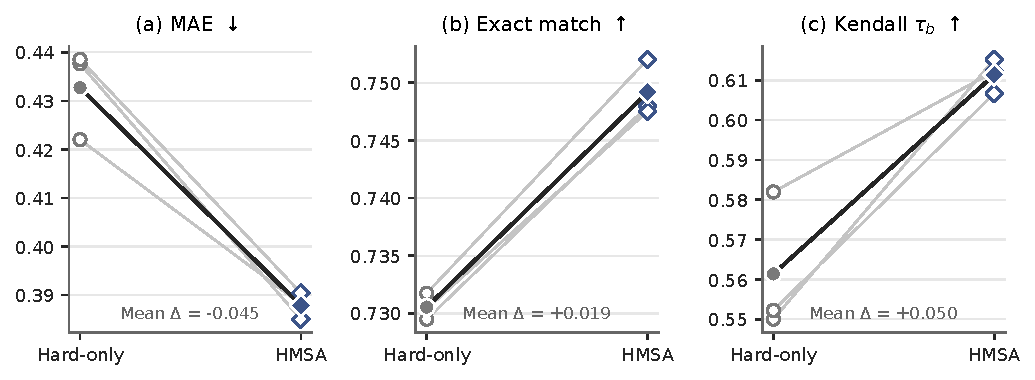
\includegraphics[width=\linewidth]{figures/fig2_seed_paired_primary.pdf}
\caption{测试集上三个随机种子的配对结果。细灰线和空心标记表示单个种子，粗黑线和实心标记表示三种子均值；灰色圆点为 Hard-only，蓝色菱形为 HMSA。三个子图使用各自的局部纵轴范围，以突出种子内配对差异；不同面板的视觉跨度不表示效应量大小。}
\label{fig:seed_pairs}
\end{figure}
\FloatBarrier

除主指标外，HMSA 将平均 L2H 严重错误数从 $59.7$ 降至 $37.3$，平均减少 $22.3$ 条；在固定的 103 个低分测试条目中，对应错误率从 $57.9\%$ 降至 $36.2\%$。有符号高估偏差从 $0.200$ 降至 $0.146$，QWK 从 $0.522$ 提升至 $0.651$，三档一致率从 0.879 提升至 0.890。这些指标并非相互独立，因此应将其视为与主指标方向一致的误差画像，而非多个独立的显著性检验。

\subsection{RQ2：收益集中于低中分等级，5 分召回轻微下降}

图\ref{fig:recall} 展示分等级召回率，精确数值见附录表\ref{tab:recall}。HMSA 对 1 分的召回从 0.155 提升至 0.440，绝对增加 0.286；2 分从 0.199 提升至 0.270；3 分从 0.297 提升至 0.351；4 分从 0.696 提升至 0.720。与此同时，5 分召回从 0.869 轻微下降至 0.864，差值为 $-0.004$。因此，不能声称“所有指标、所有等级均改善”；更准确的结论是，在三个种子的平均结果中，HMSA 在几乎不损害最高等级召回的情况下减少了对低质量回答的漏检。

\begin{figure}[H]
\centering
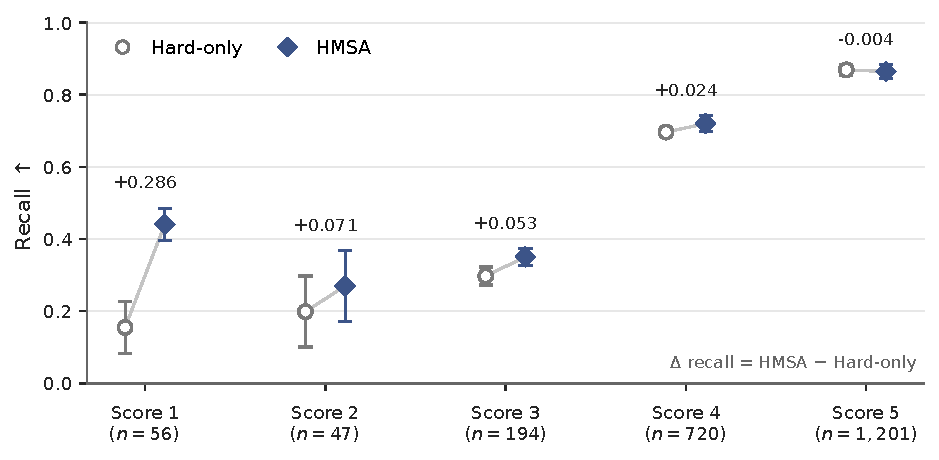
\includegraphics[width=0.84\linewidth]{figures/fig3_test_recall_by_label.pdf}
\caption{测试集分等级召回率（三种子均值）。误差条为跨训练随机种子的样本标准差而非置信区间；组上数字为 HMSA$-$Hard-only，横轴第二行给出各等级样本数。}
\label{fig:recall}
\end{figure}
\FloatBarrier

低分样本仍然是最困难的区域：即使经过提升，HMSA 对 1 分和 2 分的平均召回也只有 0.440 和 0.270。样本不平衡没有被忽略，而是被保留为部署局限；本实验刻意不引入类别权重或重采样，因为那会把“辅助分布头是否有效”的单变量问题改成新的组合实验。面向实际质量控制，后续研究仍需专门优化低分敏感度。

\subsection{RQ3：样本对应与目标表示均影响开发集增量}

Direct-soft 令同一个部署输出头直接拟合三人经验分布，Single-head mix 则在同一输出头中混合硬目标与软目标。在随机种子 42 的预设开发集门槛下，两者均未获得继续多种子评估的资格。该诊断仅说明两个固定配置未在规定门槛下推进，不代表直接软监督或单头混合这一方法家族普遍无效，也不构成逐级消融。

为避免根据测试结果追加分组分析，评分一致性分层仅在开发集上进行。附录表\ref{tab:dev_disagreement} 显示，在 291 个三人一致样本上，HMSA 的 MAE 降低 0.023、精确匹配率提高 0.017；在 373 个相邻等级 2:1 分歧样本上，MAE 降低 0.007、精确匹配率提高 0.007。QWK 在两组中均约提升 0.047，而有符号偏差在分歧组下降更多。

结果表明，收益并非只发生在分歧样本：HMSA 对一致样本同样有效，且其 MAE 改善更大。仅凭这一分层，无法区分样本级细粒度目标对应与一般多任务正则化。

表\ref{tab:dev_mechanism_summary} 给出三种子开发集机制对照。Shuffled-soft 相比 Hard-only 的平均 MAE、精确匹配率和 Kendall $\tau_b$ 分别变化 $-0.004$、$+0.003$ 和 $+0.008$，说明即使样本对应关系被破坏，类别条件软目标和双头训练本身也可能产生一定正则化收益。HMSA 在此基础上进一步将 MAE 降低 0.010，将精确匹配率和 Kendall $\tau_b$ 提高 0.009 和 0.020；附录表\ref{tab:dev_mechanism_by_seed} 显示，这三项 HMSA$-$Shuffled-soft 差值在种子 42、43 和 44 上均为有利方向。

\begin{table}[H]
\centering
\caption{事后开发集机制对照（均值 $\pm$ 跨三个训练随机种子的样本标准差）。Shuffled-soft 保留各硬标签内软目标的完整多重集，但打乱样本与软目标的对应关系；$\Delta_{\mathrm{H-S}}$ 为 HMSA$-$Shuffled-soft。}
\label{tab:dev_mechanism_summary}
\small
\setlength{\tabcolsep}{3.8pt}
\begin{tabular}{lrrrr}
\toprule
指标 & Hard-only & Shuffled-soft & HMSA & $\Delta_{\mathrm{H-S}}$ \\
\midrule
MAE $\downarrow$ & 0.393 $\pm$ 0.016 & 0.389 $\pm$ 0.009 & \textbf{0.379 $\pm$ 0.003} & -0.010 \\
精确匹配率 $\uparrow$ & 0.719 $\pm$ 0.011 & 0.722 $\pm$ 0.005 & \textbf{0.731 $\pm$ 0.005} & +0.009 \\
Kendall $\tau_b$ $\uparrow$ & 0.569 $\pm$ 0.024 & 0.577 $\pm$ 0.021 & \textbf{0.597 $\pm$ 0.007} & +0.020 \\
有符号偏差（0 最佳） & 0.150 $\pm$ 0.035 & 0.120 $\pm$ 0.032 & \textbf{0.111 $\pm$ 0.026} & -0.010 \\
QWK $\uparrow$ & 0.602 $\pm$ 0.040 & 0.635 $\pm$ 0.007 & \textbf{0.648 $\pm$ 0.016} & +0.013 \\
L2H 数量 $\downarrow$ & 11.3 $\pm$ 2.5 & \textbf{8.3 $\pm$ 0.6} & 8.7 $\pm$ 1.5 & +0.3 \\
\bottomrule
\end{tabular}
\end{table}


这一结果表明，仅增加第二个头或保留每个硬标签内的软目标组成，尚不足以解释 HMSA 在当前开发集上的全部主要指标增量；恢复训练样本与三人评分分布的原始对应关系后，三项主指标进一步改善。同时，Shuffled-soft 的均值也略优于 Hard-only，说明一般辅助正则化可能贡献部分收益。该结论不能扩展为“所有误差均由对应关系改善”：Shuffled-soft 的平均 L2H 为 8.333，略低于 HMSA 的 8.667。

表\ref{tab:dev_meanaux_summary} 给出第二项匹配对照。MeanAux 的 MAE、精确匹配率和 Kendall $\tau_b$ 分别为 $0.395\pm0.009$、$0.710\pm0.003$ 和 $0.569\pm0.006$，相对 Hard-only 分别变化 $+0.002$、$-0.009$ 和近似 0，未复现 HMSA 的开发集增量。HMSA 相比 MeanAux 分别改善 0.016、0.021 和 0.028；附录表\ref{tab:dev_meanaux_by_seed} 显示，三个差值在种子 42、43 和 44 上均为有利方向。

\begin{table}[H]
\centering
\caption{连续均分辅助目标的事后开发集匹配对照（均值 $\pm$ 跨三个训练随机种子的样本标准差）。MeanAux 与 HMSA 具有相同的双头结构和硬头评分路径，只将辅助目标及损失替换为连续人类均分与 Smooth L1。}
\label{tab:dev_meanaux_summary}
\small
\begin{tabular}{lrrr}
\toprule
配置 & MAE $\downarrow$ & 精确匹配率 $\uparrow$ & Kendall $\tau_b$ $\uparrow$ \\
\midrule
Hard-only & 0.393 $\pm$ 0.016 & 0.719 $\pm$ 0.011 & 0.569 $\pm$ 0.024 \\
MeanAux & 0.395 $\pm$ 0.009 & 0.710 $\pm$ 0.003 & 0.569 $\pm$ 0.006 \\
HMSA & \textbf{0.379 $\pm$ 0.003} & \textbf{0.731 $\pm$ 0.005} & \textbf{0.597 $\pm$ 0.007} \\
\bottomrule
\end{tabular}
\end{table}


两项对照共同缩小了解释空间：HMSA 的结果既不能完全归因于一般双头正则化，也不能由当前固定形式的连续均分辅助回归复现。由于均分与经验分布在数据中一一对应，MeanAux 的对照结果支持“目标表示与损失几何影响训练效果”，而不是“分布包含额外标签信息”。此外，MeanAux 同时将经验分布交叉熵替换为期望分数上的 Smooth L1，尚不能进一步区分优势来自五类概率约束、交叉熵梯度还是二者共同作用。两项对照均为事后开发集分析，仍需独立数据复核。

\FloatBarrier

\section{讨论与局限性}

\paragraph{为什么单头软监督没有推进，而双头配置能够推进。}
Direct-soft 将部署输出头直接训练为三人经验分布；Single-head mix 则在同一输出头中混合硬目标与软目标。两者均改变了部署逻辑值所拟合的目标。HMSA 保留软监督，但将其输出约束移至独立辅助头，使主头继续针对整数标签优化。现有结果与“部署输出上的直接目标竞争得到缓解”这一解释相容，但实验未直接测量梯度冲突、表示变化或决策边界，因而尚不能确认具体机制。

\paragraph{软头不会改变最终输出形式。}
最终输出仍为 1--5 分整数。辅助头在训练阶段为共享主干提供复现三位评分者经验分布的附加约束，但不直接更新硬头参数。即使部署时裁剪辅助头，共享主干也已受到两项损失的梯度更新。Hard-only 与 HMSA 的受控比较表明，这一训练配置与更好的硬头预测结果相关，但无法单独说明共享表示以何种方式改变。

\paragraph{机制对照缩小了什么解释空间。}
标签内置换保持双头结构和类别条件软目标组成，却使 56.14\% 的训练条目不再接收自身评分分布。Shuffled-soft 相比 Hard-only 的小幅均值收益与一般辅助正则化相容；HMSA 相比 Shuffled-soft 在三个主指标和三个种子上的一致优势，支持样本级细粒度目标对应提供增量。MeanAux 进一步保持双头容量和硬头路径，并使用与经验分布一一对应的连续均分；其未优于 Hard-only，而 HMSA 在每个种子的三个主指标上均优于 MeanAux，说明并非任意细粒度辅助目标都能复现结果。两项对照仍未直接观测梯度、表示或决策边界；“支持”不等于确认唯一机制。

\paragraph{数据与外推限制。}
研究仅使用一个 0.6B Qwen3 基座、一个教育评分数据集和一组固定划分，尚不能说明方法在其他模型家族、参数规模或教育数据上的普适性。训练集与测试集高度偏向 4--5 分，低分召回率仍然不足。评分分歧也只包含完全一致或相邻等级 2:1，结论尚未覆盖跨度更大的分歧模式。正因评分模式受限，经验分布与连续人类均分在每个划分内一一对应；MeanAux 虽提供了信息可恢复性匹配的对照，却同时改变目标参数化与损失函数，故仍不能将增益解释为分布包含均分之外的信息，也不能确定是哪一项训练几何差异产生作用。

\paragraph{统计限制。}
主要结果只有三个训练种子。均值$\pm$样本标准差展示了三个运行的变化，但不足以精确估计训练随机性的总体分布。条目级与问题簇级自助重采样均利用固定测试集上的三种子平均配对差异，不能替代更多训练种子或外部数据复核。多个辅助指标也未进行全面的多重比较校正。Shuffled-soft 与 MeanAux 均在正式测试之后提出且仅在开发集评估，其结果应视为探索性机制证据，而非独立确认性检验。

\paragraph{设计空间限制。}
辅助损失权重固定为 1.0，尚未证明最优；软头与硬头等规模且共享全部主干，也不是唯一可行结构。实验未评估梯度手术、动态权重、类别重加权或低分过采样。当前设计旨在隔离一个清晰的结构变化，而非完成整个系统空间的最优搜索。

\section{结论}

本文将软标签辅助多任务范式应用于教育五级评分，并保留硬标签主头作为唯一决策路径。相对严格匹配的 Hard-only，HMSA 在开发集和测试集上均获得三个随机种子同方向的 MAE、精确匹配率和排序改善，并减少低分到高分的严重误判。标签内置换对照支持样本级对应提供增量；连续均分辅助对照未优于 Hard-only，而 HMSA 在每个种子的三个开发集主指标上均优于该对照。5 分召回轻微下降、L2H 未优于置换对照，表明低分识别仍未充分解决。总体而言，评分分布辅助任务与硬标签部署目标在当前设定下兼容，样本对应及目标表示--损失设计均可能影响效果。现有证据不支持额外标签信息主张；具体机制仍需独立数据、更多基座与更细损失消融确认。

\FloatBarrier
\appendix

\section{补充结果与评分一致性分层}

表\ref{tab:recall} 给出测试集分等级召回率的精确数值。表\ref{tab:diagnostic_seed42} 给出单种子诊断结果，表\ref{tab:dev_disagreement} 给出评分一致性分层，表\ref{tab:dev_mechanism_by_seed} 与表\ref{tab:dev_meanaux_by_seed} 分别列出标签内置换和连续均分辅助对照的逐种子开发集结果。

\begin{table}[H]
\centering
\caption{测试集上的分等级召回率（均值 $\pm$ 跨三个训练随机种子的样本标准差）；$n$ 表示各等级样本数，差值由未四舍五入的数值计算。}
\label{tab:recall}
\small
\begin{tabular}{rrrrr}
\toprule
评分等级 & $n$ & Hard-only & HMSA & $\Delta$ \\
\midrule
1 & 56 & 0.155 $\pm$ 0.072 & \textbf{0.440 $\pm$ 0.045} & +0.286 \\
2 & 47 & 0.199 $\pm$ 0.098 & \textbf{0.270 $\pm$ 0.098} & +0.071 \\
3 & 194 & 0.297 $\pm$ 0.025 & \textbf{0.351 $\pm$ 0.024} & +0.053 \\
4 & 720 & 0.696 $\pm$ 0.012 & \textbf{0.720 $\pm$ 0.022} & +0.024 \\
5 & 1,201 & \textbf{0.869 $\pm$ 0.015} & 0.864 $\pm$ 0.020 & -0.004 \\
\bottomrule
\end{tabular}
\end{table}


\begin{table}[H]
\centering
\caption{开发集随机种子 42 的诊断结果。Direct-soft 与 Single-head mix 仅用于预设推进判定；“未推进”表示未通过门槛，不代表相应方法族普遍无效。}
\label{tab:diagnostic_seed42}
\small
\begin{tabular}{lrrrrrrl}
\toprule
配置 & 轮次 & MAE $\downarrow$ & 精确匹配率 $\uparrow$ & Kendall $\tau_b$ $\uparrow$ & 有符号偏差 & L2H & 结论 \\
\midrule
Hard-only & 8 & 0.386 & 0.718 & 0.577 & +0.114 & 11 & 基线 \\
Direct-soft & 5 & 0.389 & 0.714 & 0.576 & +0.102 & 8 & 未推进 \\
Single-head mix & 6 & 0.384 & 0.718 & 0.590 & +0.102 & 8 & 未推进 \\
HMSA & 5 & 0.377 & 0.729 & 0.605 & +0.094 & 7 & 推进 \\
\bottomrule
\end{tabular}
\end{table}


\begin{table}[H]
\centering
\caption{开发集上的评分一致性分层分析（均值 $\pm$ 跨三个训练随机种子的样本标准差）。}
\label{tab:dev_disagreement}
\small
\begin{tabular}{llrrrr}
\toprule
分组 & 指标 & $n$ & Hard-only & HMSA & $\Delta$ \\
\midrule
三人一致 & MAE & 291 & 0.251 $\pm$ 0.031 & \textbf{0.228 $\pm$ 0.002} & -0.023 \\
 & 精确匹配率 &  & 0.817 $\pm$ 0.019 & \textbf{0.834 $\pm$ 0.005} & +0.017 \\
 & 有符号偏差 &  & 0.134 $\pm$ 0.027 & \textbf{0.111 $\pm$ 0.015} & -0.023 \\
 & QWK &  & 0.654 $\pm$ 0.065 & \textbf{0.700 $\pm$ 0.017} & +0.047 \\
\midrule
相邻等级2:1分歧 & MAE & 373 & 0.504 $\pm$ 0.013 & \textbf{0.497 $\pm$ 0.005} & -0.007 \\
 & 精确匹配率 &  & 0.643 $\pm$ 0.018 & \textbf{0.651 $\pm$ 0.009} & +0.007 \\
 & 有符号偏差 &  & 0.163 $\pm$ 0.040 & \textbf{0.111 $\pm$ 0.036} & -0.052 \\
 & QWK &  & 0.529 $\pm$ 0.030 & \textbf{0.576 $\pm$ 0.018} & +0.047 \\
\bottomrule
\end{tabular}
\end{table}


\begin{table}[H]
\centering
\caption{事后开发集机制对照的逐种子结果。轮次表示按相同开发集精确匹配率规则选出的检查点；三个主指标均只读取硬标签主头。}
\label{tab:dev_mechanism_by_seed}
\small
\begin{tabular}{clrrrr}
\toprule
种子 & 配置 & 轮次 & MAE $\downarrow$ & 精确匹配率 $\uparrow$ & Kendall $\tau_b$ $\uparrow$ \\
\midrule
42 & Hard-only & 8 & 0.386 & 0.718 & 0.577 \\
 & Shuffled-soft & 5 & 0.388 & 0.723 & 0.587 \\
 & HMSA & 5 & \textbf{0.377} & \textbf{0.729} & \textbf{0.605} \\
\addlinespace[2pt]
43 & Hard-only & 3 & 0.411 & 0.709 & 0.542 \\
 & Shuffled-soft & 10 & 0.399 & 0.717 & 0.553 \\
 & HMSA & 10 & \textbf{0.382} & \textbf{0.727} & \textbf{0.593} \\
\addlinespace[2pt]
44 & Hard-only & 5 & 0.382 & 0.730 & 0.588 \\
 & Shuffled-soft & 5 & 0.382 & 0.727 & 0.590 \\
 & HMSA & 6 & \textbf{0.379} & \textbf{0.736} & \textbf{0.592} \\
\bottomrule
\end{tabular}
\end{table}


\begin{table}[H]
\centering
\caption{连续均分辅助目标对照的逐种子开发集结果。轮次由硬头开发集精确匹配率选择；所有指标均只读取硬头。}
\label{tab:dev_meanaux_by_seed}
\small
\begin{tabular}{clrrrr}
\toprule
种子 & 配置 & 轮次 & MAE $\downarrow$ & 精确匹配率 $\uparrow$ & Kendall $\tau_b$ $\uparrow$ \\
\midrule
42 & Hard-only & 8 & 0.386 & 0.718 & 0.577 \\
 & MeanAux & 8 & 0.389 & 0.708 & 0.576 \\
 & HMSA & 5 & \textbf{0.377} & \textbf{0.729} & \textbf{0.605} \\
\addlinespace[2pt]
43 & Hard-only & 3 & 0.411 & 0.709 & 0.542 \\
 & MeanAux & 6 & 0.405 & 0.709 & 0.565 \\
 & HMSA & 10 & \textbf{0.382} & \textbf{0.727} & \textbf{0.593} \\
\addlinespace[2pt]
44 & Hard-only & 5 & 0.382 & 0.730 & 0.588 \\
 & MeanAux & 5 & 0.392 & 0.714 & 0.566 \\
 & HMSA & 6 & \textbf{0.379} & \textbf{0.736} & \textbf{0.592} \\
\bottomrule
\end{tabular}
\end{table}


\FloatBarrier

\section{可复核性材料}

随附复核材料的 \texttt{data/} 目录包含由锁定报告机械导出的 CSV 和 JSON，\texttt{scripts/} 目录包含数据导出、制表、绘图与附加审计脚本。测试结果导出脚本只读取已锁定的指标与规范化报告，不重新读取原始测试数据。规范化报告同时记录六个模型检查点、预测向量、指标文件和最终清单的 SHA-256 哈希。问题簇自助重采样脚本读取六份冻结测试预测，仅从锁定测试划分恢复问题标识并以问题为重采样单位；均分--分布对应审计脚本则分别核验训练集、开发集和测试集中的对应关系。标签内置换对照另提供三方案汇总、逐种子指标与置换审计。MeanAux 报告记录统一源码锁、三个互异的种子级检查点目录与预测哈希，并确认测试访问计数为 0。正文除明确标注的 $\Delta_{\mathrm{H-S}}$ 外，方法差值统一定义为 HMSA$-$Hard-only；因此 MAE、有符号偏差与 L2H 为负表示改善，精确匹配率、Kendall $\tau_b$ 和 QWK 为正表示改善。实验日志未保存精确依赖、模型快照与 GPU 型号；该缺口将在发布材料中保留。

\begin{thebibliography}{99}

\bibitem{caruana1997multitask}
Caruana, R. Multitask learning. \emph{Machine Learning}, 28:41--75, 1997.

\bibitem{davani2022}
Mostafazadeh Davani, A., Díaz, M., and Prabhakaran, V. Dealing with disagreements: Looking beyond the majority vote in subjective annotations. \emph{Transactions of the Association for Computational Linguistics}, 10:92--110, 2022.

\bibitem{fornaciari2021}
Fornaciari, T., Uma, A., Paun, S., Plank, B., Hovy, D., and Poesio, M. Beyond black \& white: Leveraging annotator disagreement via soft-label multi-task learning. In \emph{Proceedings of NAACL-HLT}, pp. 2591--2597, 2021.

\bibitem{gu2024survey}
Gu, J., Jiang, X., Shi, Z., et al. A survey on LLM-as-a-judge. arXiv preprint arXiv:2411.15594, 2024.

\bibitem{kurniawan2026}
Kurniawan, K., Mistica, M., Baldwin, T., and Lau, J. H. Training and evaluating with human label variation: An empirical study. \emph{Computational Linguistics}, 52(1):85--111, 2026.

\bibitem{lewidi2021}
Uma, A., Fornaciari, T., Dumitrache, A., et al. SemEval-2021 Task 12: Learning with disagreements. In \emph{Proceedings of SemEval-2021}, pp. 338--347, 2021.

\bibitem{lewidi2023}
Leonardelli, E., Abercrombie, G., Almanea, D., et al. SemEval-2023 Task 11: Learning with disagreements (LeWiDi). In \emph{Proceedings of SemEval-2023}, pp. 2304--2318, 2023.

\bibitem{li2024llmjudge}
Li, H., Dong, Q., Chen, J., et al. LLMs-as-judges: A comprehensive survey on LLM-based evaluation methods. arXiv preprint arXiv:2412.05579, 2024.

\bibitem{macina2025mathtutorbench}
Macina, J., Daheim, N., Hakimi, I., Kapur, M., Gurevych, I., and Sachan, M. MathTutorBench: A benchmark for measuring open-ended pedagogical capabilities of LLM tutors. In \emph{Proceedings of EMNLP}, pp. 204--221, 2025.

\bibitem{maurya2025mrbench}
Maurya, K. K., Srivatsa, K. A., Petukhova, K., and Kochmar, E. Unifying AI tutor evaluation: An evaluation taxonomy for pedagogical ability assessment of LLM-powered AI tutors. In \emph{Proceedings of NAACL-HLT}, pp. 1234--1251, 2025.

\bibitem{peterson2019human}
Peterson, J. C., Battleday, R. M., Griffiths, T. L., and Russakovsky, O. Human uncertainty makes classification more robust. In \emph{Proceedings of ICCV}, 2019.

\bibitem{plank2022}
Plank, B. The problem of human label variation: On ground truth in data, modeling and evaluation. In \emph{Proceedings of EMNLP}, pp. 10671--10682, 2022.

\bibitem{prioraudit}
Anonymous. Auditing large language models as educational assistants and judges. Manuscript under anonymous review, 2026.

\bibitem{qwen3embedding}
Zhang, Y., Li, M., Long, D., et al. Qwen3 Embedding: Advancing text embedding and reranking through foundation models. arXiv preprint arXiv:2506.05176, 2025.

\bibitem{uma2021learning}
Uma, A., Fornaciari, T., Hovy, D., Paun, S., Plank, B., and Poesio, M. Learning from disagreement: A survey. \emph{Journal of Artificial Intelligence Research}, 72:1385--1470, 2021.

\bibitem{wang2025overconfidence}
Tian, Z., Han, Z., Chen, Y., Xu, H., Yang, X., Xuan, R., Wang, H., and Liao, L. Overconfidence in LLM-as-a-judge: Diagnosis and confidence-driven solution. arXiv preprint arXiv:2508.06225, 2025.

\bibitem{edubench}
Xu, B., Bai, Y., Sun, H., Lin, Y., Liu, S., Liang, X., Li, Y., Dong, Z., Zhang, J., Deng, Y., Zou, X., Gao, Y., and Huang, H. EduBench: A comprehensive benchmarking dataset for evaluating large language models in diverse educational scenarios. In \emph{Proceedings of the 64th Annual Meeting of the Association for Computational Linguistics (Volume 1: Long Papers)}, pp. 21615--21645, 2026.

\bibitem{zheng2023mtbench}
Zheng, L., Chiang, W.-L., Sheng, Y., et al. Judging LLM-as-a-judge with MT-Bench and Chatbot Arena. In \emph{Advances in Neural Information Processing Systems}, 2023.

\end{thebibliography}

\end{document}
